\documentclass[]{book}
\usepackage{lmodern}
\usepackage{amssymb,amsmath}
\usepackage{ifxetex,ifluatex}
\usepackage{fixltx2e} % provides \textsubscript
\ifnum 0\ifxetex 1\fi\ifluatex 1\fi=0 % if pdftex
  \usepackage[T1]{fontenc}
  \usepackage[utf8]{inputenc}
\else % if luatex or xelatex
  \ifxetex
    \usepackage{mathspec}
  \else
    \usepackage{fontspec}
  \fi
  \defaultfontfeatures{Ligatures=TeX,Scale=MatchLowercase}
\fi
% use upquote if available, for straight quotes in verbatim environments
\IfFileExists{upquote.sty}{\usepackage{upquote}}{}
% use microtype if available
\IfFileExists{microtype.sty}{%
\usepackage[]{microtype}
\UseMicrotypeSet[protrusion]{basicmath} % disable protrusion for tt fonts
}{}
\PassOptionsToPackage{hyphens}{url} % url is loaded by hyperref
\usepackage[unicode=true]{hyperref}
\hypersetup{
            pdftitle={Space Invaders - IA},
            pdfauthor={Ivan de Jesus Pereira Pinto},
            pdfborder={0 0 0},
            breaklinks=true}
\urlstyle{same}  % don't use monospace font for urls
\usepackage{natbib}
\bibliographystyle{apalike}
\usepackage{longtable,booktabs}
% Fix footnotes in tables (requires footnote package)
\IfFileExists{footnote.sty}{\usepackage{footnote}\makesavenoteenv{long table}}{}
\usepackage{graphicx,grffile}
\makeatletter
\def\maxwidth{\ifdim\Gin@nat@width>\linewidth\linewidth\else\Gin@nat@width\fi}
\def\maxheight{\ifdim\Gin@nat@height>\textheight\textheight\else\Gin@nat@height\fi}
\makeatother
% Scale images if necessary, so that they will not overflow the page
% margins by default, and it is still possible to overwrite the defaults
% using explicit options in \includegraphics[width, height, ...]{}
\setkeys{Gin}{width=\maxwidth,height=\maxheight,keepaspectratio}
\IfFileExists{parskip.sty}{%
\usepackage{parskip}
}{% else
\setlength{\parindent}{0pt}
\setlength{\parskip}{6pt plus 2pt minus 1pt}
}
\setlength{\emergencystretch}{3em}  % prevent overfull lines
\providecommand{\tightlist}{%
  \setlength{\itemsep}{0pt}\setlength{\parskip}{0pt}}
\setcounter{secnumdepth}{5}
% Redefines (sub)paragraphs to behave more like sections
\ifx\paragraph\undefined\else
\let\oldparagraph\paragraph
\renewcommand{\paragraph}[1]{\oldparagraph{#1}\mbox{}}
\fi
\ifx\subparagraph\undefined\else
\let\oldsubparagraph\subparagraph
\renewcommand{\subparagraph}[1]{\oldsubparagraph{#1}\mbox{}}
\fi

% set default figure placement to htbp
\makeatletter
\def\fps@figure{htbp}
\makeatother

\usepackage{booktabs}
\usepackage{amsthm}

%encoding
%--------------------------------------
\usepackage[T1]{fontenc}
\usepackage[utf8]{inputenc}
%--------------------------------------

%Portuguese-specific commands
%--------------------------------------
\usepackage[brazil]{babel}
%--------------------------------------
\makeatletter
\def\thm@space@setup{%
  \thm@preskip=8pt plus 2pt minus 4pt
  \thm@postskip=\thm@preskip
}
\makeatother

\title{Space Invaders - IA}
\author{Ivan de Jesus Pereira Pinto}
\date{2020-02-13}

\begin{document}
\maketitle

{
\setcounter{tocdepth}{1}
\tableofcontents
}
\chapter*{Resumo}\label{resumo}
\addcontentsline{toc}{chapter}{Resumo}

\begin{center}\rule{0.5\linewidth}{0.5pt}\end{center}

\begin{center}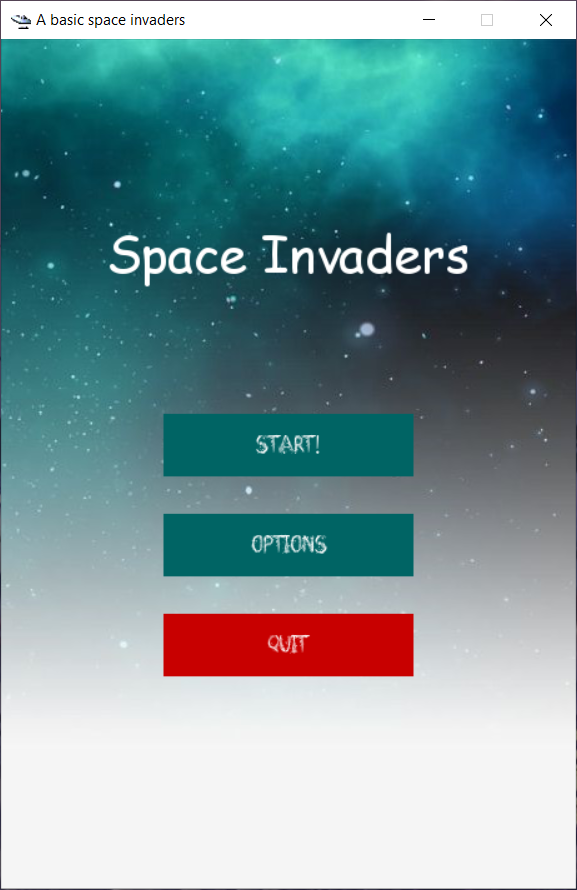
\includegraphics[width=0.5\linewidth]{content/imgs/game} \end{center}

Neste relatório descrevemos as técnicas utilizadas nos agentes do jogo
\emph{space invaders}, além do processo de treinamento.

\chapter{Introdução}\label{intro}

Esse projeto visa o desenvolvimento de técnicas da área de Inteligência
Artificial para o jogo de Space Invaders. Especificamente almeja-se a
implementação de IAs para as naves inimigas. A maior parte da pesquisa
nessa área se dá no desenvolvimento de Agentes que aprendem a jogar
contra o ambiente, no estilo de um processo de decisão de Markov
conforme ilustramos na Figura \ref{fig:pdm}:

\begin{figure}

{\centering 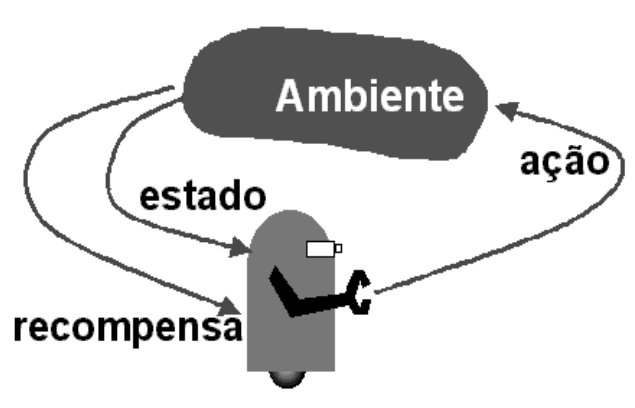
\includegraphics[width=0.5\linewidth]{content/imgs/agente-ambiente} 

}

\caption{Processo de decisão de markov. [@faria1999explorando]}\label{fig:pdm}
\end{figure}

O SpaceInvaders aqui desenvolvido almeja no entanto politicas de
controle para o ambiente, que seriam os inimigos. O jogador(humano) se
torna o ambiente nesse caso. Para que fosse possível a implementação das
técnicas de IA, foi necessário o desenvolvimento do jogo, de um
simulador, e de um surrogate para o jogador. Os objetivos deste trabalho
são listados a seguir:

\begin{enumerate}
\def\labelenumi{\arabic{enumi}.}
\tightlist
\item
  Construção do jogo de Space Invaders eficiente em C.
\item
  Construção de um Forward Simulator
\item
  Desenvolvimento de um surrugate Player que substitua o humano em tempo
  de planning ou treino.
\item
  Implementação de Técnicas de IA (Planning e Aprendizado)
\end{enumerate}

\chapter{Desafio}\label{desafio}

O jogo de Space Invaders tem 2 principais desafios: o primeiro é, como
vários jogos similares, o número enorme de estados possível, tornando
inviável a utilização de métodos exatos ou programação dinâmica para
computar a política ótima. O segundo problema, mais particular ao jogo,
é o fato de que o agente controla as naves oponentes, aumentando assim o
espaço de ações enormemente. Dado que nessa versão do jogo os oponentes
tem 5 ações possíveis, 4 direções e tiro, e temos 3 oponentes, o número
de ações possíveis vai ser 5\emph{5}5 = 125 ações. O número pequeno de
oponentes é proposital, pois o espaço de ações cresce muito, tornando
inviável as técnicas aqui descritas. Versões mais eficientes estão em
desenvolvimento.

\chapter{Surrogate Player}\label{surrogate-player}

Para que as técnicas de IA sejam viáveis, é necessário a interação com
um jogador. No entanto, essa é uma questão difícil, já que é custoso o
tempo disponível de um humano. A solução é então fazermos um modelo do
jogador humano, um \emph{surrogate}. Com este propósito, as técnicas de
planning são uma forma de se construir esse surrogate, já que diferente
de modelos black box, elas são intuitivas e entendíveis, permitindo o
debug e aprimoramento dos modelos. Nesse projeto foi utilizada a máquina
de estados finito(FSM) para modelar o comportamento do jogador humano. O
diagrama abaixo demonstra o funcionamento da FSM:

\begin{figure}

{\centering 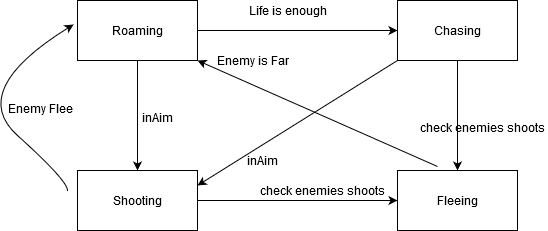
\includegraphics[width=0.5\linewidth]{content/imgs/FSM} 

}

\caption{Diagrama FSM}\label{fig:fsm}
\end{figure}

Os estados são os seguintes: Roaming,Shooting, Chasing, Fleeing. No
Roaming, a fsm ficar verificando as condições para mudar de estado. Ele
vai para shooting caso o oponente esteja em sua mira(checando as
corrdenadas na vertical). Chasing é se tendo uma quantidade significante
de vida, a fsm persegue o oponente mais próximo. Fleeing é quando sua
vida for muito baixa, em comparação ao inimigos.

\chapter{Metodologia}\label{methods}

Descrevemos aqui os métodos utilizados neste projeto. Importante: a
recompensa é +1 pra cada dano recebido pela nave do jogador( do ponto de
vista dos oponente, os quais estamos tentanto otimizar) e -1 pra cada
dano recebido pela nave oponente. Além disso, +100 é dado de o tiro
inimigo matar o oponente, e -100 é recebido se uma nave inimiga morrer.

\section{Neural Network}\label{neural-network}

Uma rede neural de 1 camada escondida foi treinada com busca aleatória
no espaço de pesos. O processo é muito simples, com a rede sendo
avaliada em um número de partidas com os pesos gerados, e caso ela seja
a melhor rede até agora( no acúmulo de recompensas), salvamos seus pesos
e os modificamos em direções aleatória usando ruído gaussiano. O
resultado foi aquém do esperado, talvez devido a complexidade do
problema e a esparcidade das recompensas, que ocorrem com pouca
frequência.

\section{Monte Carlo 1-Step Planning}\label{monte-carlo-1-step-planning}

Utiliza-se simulação monte carlo para se estimar o retorno esperado de
cada ação possível no estado atual. Rollouts/playouts/partidas
aleatórias são simuladas até certo passo estipulado. A recompensa
acumulada até aquele passo é utilizada como estimativa do retorno
esperado. Quanto mais simulações melhor, logo é importante a velocidade
do simulador. O funcionamento é ilustrado na figura abaixo:

\begin{center}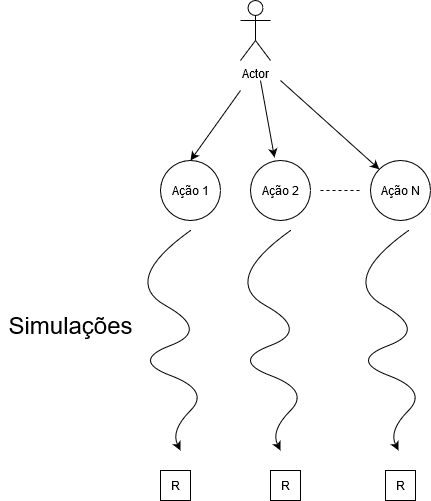
\includegraphics[width=0.5\linewidth]{content/imgs/MC} \end{center}

Por causa do enorme número de ações, esse método se torna menos
eficiente. Melhorias possíveis são a utilização de métodos que
selecionam subconjuntos de ações disponíveis.

\section{Monte Carlo Tree Search}\label{monte-carlo-tree-search}

O MCTS \citep{browne2012survey} é o método de melhor resultado, é uma
melhoria do MC onde se constroi uma árvore de ações na memória. Seu
funcionamento se dá pelos 4 passos ilustrados na figura abaixo:

\begin{center}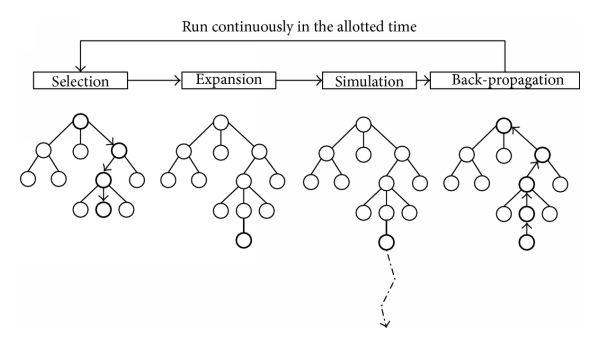
\includegraphics[width=0.5\linewidth]{content/imgs/MCTS} \end{center}

Selection: O agente percorre a parte da árvore na memória, escolhendo os
nós por meio do UCB, umas das técnicas de tomada de decisão do problema
de Multi-armed bandit. Expansion: Dentre os nós filhos do ultimo nó da
seleção, escolhemos um para colocar na memória. Geralmente a escolha é
sequencial. Playout: O jogo continua de modo aleatório até o fim da
partida Backpropagation: As recompensas são adicionadas aos nós da
memória percorridos nessa iteração.

A MCTS vai acabar convergindo na arvore de busca MinMax, que encontra a
melhor decisão considerando o as melhores decisões que o oponente pode
tomar(Equilíbrio Nash). No entanto, é importante frisar que as ações do
jogador vem de um surrogate, o que diminui a validade téorica do
algoritmo.

\chapter{Aplicação}\label{app}

\section{Instalaçao}\label{instalauxe7ao}

git clone no repositório:
\url{https://github.com/abcp4/SpaceInvaders.git}

Para instalar no Windows é necessário um compilador de c(gcc foi
utilizado no desenvolvimento), e de python 3.6 de 32 bits. Utilizando o
anaconda basta criar um ambiente como se segue:

Colocar variável de ambiente: set CONDA\_FORCE\_32BIT=1

Criar ambiente: conda create -n py36\_32 python=3.6

Ativar ambiente: conda activate py36\_32

Instalar numpy e pygame: pip install numpy,pygame

As depedências do python devem ter sido satisfeitas. O programa com UI
vai precisar chamar o jogo SpaceInvaders em C, para que possa funcionar.
Temos que compilar o código em C com o comando a seguir, da pasta
SpaceInvaders

gcc -Wall -fPIC -shared src/Space.c src/list.c src/genann.c -o
src/Space.so

Se tudo tiver dado certo, o jogo deve funcionar. Basta utilizar python
menu.py

\section{Jogo}\label{jogo}

O Jogo Space invaders foi desenvolvido em C de modo a ser o mais
eficiente possível. Além disso, foram utilizadas estruturas de dados com
menor complexidade, como por exemplo:

\begin{enumerate}
\def\labelenumi{\arabic{enumi}.}
\item
  o uso de Matriz para representar o espaço do jogo, tendo O(1) para
  checar se a nave do jogador ou dos oponentes receberam dados dos
  tiros.
\item
  O(n) para mover os tiros, onde n é a quantidade de tiros ativos na
  tela, armazenados em uma lista. Tiros fora da tela são descartados
\end{enumerate}

Um foward simulator foi implementado para permitir que os agentes possam
fazer simulações, para planning e treinamento.

Os comandos para jogar são os seguintes: direcionais movem a nave, e
espaço atira.

O Vídeo abaixo demonstra uma partida rapida de um humano contra a IA
MCTS

\chapter{Considerações finais}\label{considerauxe7uxf5es-finais}

Esse projeto é ainda um protótipo de um projeto maior: Permitir que o
designer do jogo possa testar, de maneira rápida e eficiente, diferentes
políticas e comportamentos dos oponentes do jogador humano. Neste
trabalho foi desenvolvido um surrogate do jogador humano com planning, e
acreditamos ser uma forma eficiente de tratar esse problema, por ser
entendivel, intuitivo, e mais importante, verificável, até para
melhorias. As técnicas para controle dos oponentes são básicas ainda,
mas já estão sendo exploradas algumas mais avançadas, como versões de
algoritmos genéticos que buscam no espaço de comportamentos(RHEA e Map
of Elits). O propósito final deste trabalho é a publicação de um paper
descrevendo os avanços alcançados.

\bibliography{references.bib,packages.bib}

\end{document}
